\chapter{Results}

\label{ch5_RESULTS}
{\bf Data set - } All experiments in this project are performed on standard Hollywood2 (actions) 
\cite{hollywood2} data set from \cite{actionsInContext}. 
It has 823 labeled training video clips and 884 labeled testing video clips. 
There are 12 activity classes : AnswerPhone, DriveCar, Eat, FightPerson,
 GetOutCar, HandShake, HugPerson, Kiss, Run, SitDown, SitUp, StandUp.
 Each clip is 10 to 30 seconds long. Frame rate is 24 fps.
 Each clip is provided with a true label. Few of the clips have multiple labels, in this project, only single labelled clips are used.


 \section{Methodology}
 \label{section_METHODOLOGY}
 {\bf Video recognizer setup - } 100,000 HoG-HoF feature vectors are randomely sampled from 
 set of all feature vectors extracted from video clips using \cite{stipCode}.
 While doing random sampling, each clip is given equal chance - this avoids biased sampling
towards (or against) any particular class of videos if they happen to be longer (or shorter) than other videos on an average.
These randomely sampled descriptors are clustered in $k = 200$ clusters using k-means.
All clips are represented in Bag-of-Features representation over these clusters as explained in section \ref{section_BOF}.

~\\
{\bf SVM - } Matlab interface of libsvm \cite{libsvm} is used to train 
12 one-vs-rest (ovr) models corresponding to 12 activity classes. A RBF kernel is used with parameters, $\gamma = 0.01$ and $C = 100$.

~\\
{\bf Object Detector Setup - } Object detector explained in section \ref{section_OBJDET} is used. 
This run of object detection has a threshold of -0.9. 
Object specific thresholding is done at a later stage while forming evidence for MLN.

The visual output of object detector looks as shown in figures \ref{fig:CarDetection} and \ref{fig:PersonDetection}. 
The boxes are called as bounding boxes.
For each box, a confidence value is also evaluated.
Table \ref{table:ObjDetection} shows sample confidence output.

\floatstyle{plain}
\restylefloat{figure}
\begin{figure}[here]
\begin{center} 
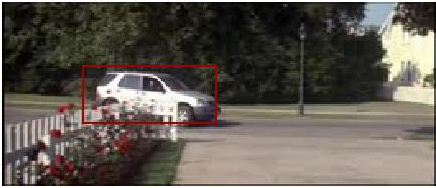
\includegraphics[scale=0.5]{car_detection_1.jpg} 
\caption{ Car detection in a frame. \label{fig:CarDetection}} 
\end{center} 
\end{figure}  

\begin{figure}[here]
\begin{center} 
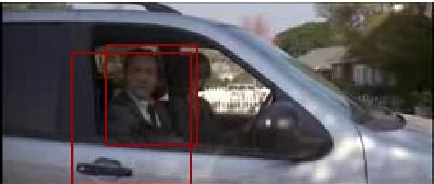
\includegraphics[scale=0.5]{person_detection_151.jpg} 
\caption{ Person detection in a frame. \label{fig:PersonDetection}} 
\end{center} 
\end{figure}  

\begin{table}[t,here]
\centering
\begin{tabular}{|l|c|}
\hline
\multicolumn{2}{|c|}{FRAME1} \\
\hline
 Car            &-0.181786\\
\hline
\multicolumn{1}{|c|}\vdots & \vdots \\
\hline
\multicolumn{1}{|c|}\vdots & \vdots \\
\hline
\multicolumn{2}{|c|}{FRAME151} \\
\hline
Person	&0.579786\\
\hline
Person	&-0.593087\\
\hline
\end{tabular}
\caption{Output of object detector with decision values}
\label{table:ObjDetection}
\end{table}

~ \\
{\bf Alchemy Setup - } MLN model is learnt using Alchemy 2.0 \cite{alchemy2.0} software.
All the parameters are kept default. `QueryEvidence' option is not set.

~\\
{\bf Classification metric - } Predictions are compared by taking \index{Average Average Precision|see {AAP}} average average precision as a measure.
As explained in \cite{actionsInContext}, average precision(AP) approximates area under recall-precision curve.
Thus, AP for each activity class is calculated and then finally averaged over all the classes, average AP (\index{AAP}AAP) is calculated.
AP is taken as a measure of performance in the work of \cite{actionsInContext}.

\section{Precision Comparisons}
{\bf MLN - } Using alchemy 2.0 \cite{alchemy2.0} software, various experiments were performed 
to add the object and people information to the existing video recognizer. 

\begin{table}[t,here]
\centering
\captionsetup{justification=centering,margin=2cm}
\begin{tabular}{| l | c | c | c | c | c |}
\hline
	{\bf Activity Class} & {\centering {\bf SVM}}
	&\multicolumn{4}{c|}{\centering {\bf MLN} }\\ \hline

	~ & ~
	& \multicolumn{1}{p{1.2cm}|}{\centering {\bf Only \\ Action}}
	& \multicolumn{1}{p{1.2cm}|}{\centering {\bf Action \& \\ Object}}
	& \multicolumn{1}{p{1.2cm}|}{\centering {\bf Action \& \\ People}}
	& \multicolumn{1}{p{1.2cm}|}{\centering {\bf Action \\ Object \& \\ People}}
	\\ \hline
	AnswerPhone	& 11.36\%  & 10.64\%  & 11.11\%  & 11.67\%  & 12.73\%  \\ \hline
	DriveCar  	& 66.96\%  & 66.06\%  & 66.67\%  & 71.57\%  & 68.18\%  \\ \hline
	Eat  		& 45.45\%  & 32.50\%  & 40.00\%  & 35.00\%  & 40.00\%  \\ \hline
	FightPerson  	& 57.63\%  & 56.90\%  & 54.84\%  & 61.54\%  & 62.26\%  \\ \hline
	GetOutCar  	& 17.86\%  & 8.00\%   & 13.79\%  & 17.39\%  & 14.29\%  \\ \hline
	HandShake  	& 25.93\%  & 21.43\%  & 25.00\%  & 30.77\%  & 41.67\%  \\ \hline
	HugPerson  	& 15.15\%  & 15.79\%  & 13.79\%  & 14.29\%  & 16.13\%  \\ \hline
	Kiss  		& 18.18\%  & 18.07\%  & 19.78\%  & 19.79\%  & 20.65\%  \\ \hline
	Run  		& 38.78\%  & 36.42\%  & 41.48\%  & 40.32\%  & 42.15\%  \\ \hline
	SitDown  	& 40.96\%  & 38.10\%  & 35.56\%  & 34.78\%  & 39.56\%  \\ \hline
	SitUp  		& 5.26\%   & 0.00\%   & 5.26\%   & 0.00\%   & 12.50\%  \\ \hline
	StandUp  	& 35.20\%  & 38.46\%  & 36.29\%  & 38.26\%  & 36.24\%  \\ \hline
	AAP  		& 31.56\%  & 28.53\%  & 30.30\%  & 31.28\%  & 33.86\%  \\ \hline

\end{tabular}
\caption{MLN Experiments - Average precisions}
\label{table:MLN_RESULTS}
\end{table}



TODO - Explanation of above table.



~\\

{\bf TF-IDF Features - }
The Bag-of-Features vector of each clip can be appended with Term Frequency -
Inverse Document Frequency (tf-idf) features corresponding 
to 12 objects and number of people information. Thus adding 13 more features to each
feature vector.
These new feature vectors are now used to learn SVM model with similar parameters 
and methodology explained in section \ref{section_METHODOLOGY}.
It shows significant improvemnt as described in table \ref{table:SVM_TFIDF}.

\begin{table}[t,here]
\centering
\captionsetup{justification=centering,margin=2cm}
\begin{tabular}{| l | c | c |}
\hline
	{\bf Activity Class}
	& \multicolumn{1}{p{3cm}|}{\centering {\bf AP - Basic \\ SVM}}
	& \multicolumn{1}{p{3cm}|}{\centering {\bf AP - Object \\ and People} }\\ \hline
AnswerPhone & 11.36\% & 16.67\% \\ \hline
DriveCar & 66.96\% & 70.09\% \\ \hline
Eat & 45.45\% & 50.00\% \\ \hline
FightPerson & 57.63\% & 66.04\% \\ \hline
GetOutCar & 17.86\% & 12.12\% \\ \hline
HandShake & 25.93\% & 31.82\% \\ \hline
HugPerson & 15.15\% & 17.86\% \\ \hline
Kiss & 18.18\% & 20.69\% \\ \hline
Run & 38.78\% & 39.35\% \\ \hline
SitDown & 40.96\% & 42.05\% \\ \hline
SitUp & 5.26\% & 8.70\% \\ \hline
StandUp & 35.20\% & 37.88\%\\ \hline
Average AP & 31.56\% & 34.44\% \\ \hline
%
\end{tabular}
\caption{Average precision after adding tf-idf features}
\label{table:SVM_TFIDF}
\end{table}

TODO - Comparison between tf-idf and MLN. Feedback.

\begin{comment}
Table \ref{table:SVM_Setup} shows APs for all classes as per SVM setup of this project.

\begin{table}[t,here]
\centering
\captionsetup{justification=centering,margin=2cm}
\begin{tabular}{| l | c | c |}
\hline
{\bf Activity Class} & {\bf AP as per Paper} & {\bf AP as per project} \\ \hline
%
AnswerPhone & 8.80\% & 11.36\% \\ \hline
DriveCar & 74.90\% & 66.96\% \\ \hline
Eat & 26.30\% & 45.45\% \\ \hline
FightPerson & 67.50\% & 57.63\% \\ \hline
GetOutCar & 9.00\% & 17.86\% \\ \hline
HandShake & 11.60\% & 25.93\% \\ \hline
HugPerson & 13.50\% & 15.15\% \\ \hline
Kiss & 49.60\% & 18.18\% \\ \hline
Run & 53.70\% & 38.78\% \\ \hline
SitDown & 31.60\% & 40.96\% \\ \hline
SitUp & 7.20\% & 5.26\% \\ \hline
StandUp & 35\% & 35.20\% \\ \hline
Average AP & 32.39\% & 31.56\% \\ \hline
%
\end{tabular}
\caption{Average precision for Basic SVM Setup - without using tf-idf features}
\label{table:SVM_Setup}
\end{table}
\end{comment}
